\chapter{Aspects techniques}

	\section{Librairie piecesPuzzle}

        Pour la conception de ce projet, une librairie a été créer, réferencant ainsi toutes les pièces possibles. Cette librairie comporte 4 pièces différentes qui ont toutes une grille créer a partir de la rotation défini.
        Cette création se fait à l'aide de la méthode \underline{\textit{createGrid()}} (présent dans la classe abstraite \textbf{AbstractPiece}) qui prend en paramètre un numéro (de 0 à 3) qui correspond a la rotation dans le sens horaire. Cette méthode change la largeur/longueur de la pièce, en prenant en compte la rotation ainsi que la largeur/longueur donnée à la pièce dans le constructeur. Ainsi, cela permet la création d'une nouvelle grille en prenant en compte la rotation. En effet, si la pièce tourne, sa largeur et longueur sont inverser, puis les valeurs sont utiliser dans la méthode \underline{\textit{pieceGrid()}} de la pièce afin de créer une nouvelle grille.

        \begin{figure}[H]
			\centering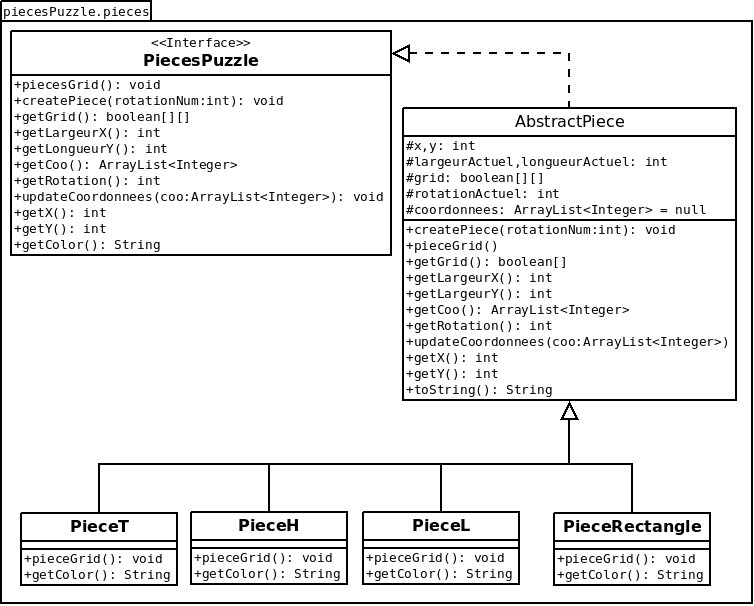
\includegraphics[width=0.64\textwidth, keepaspectratio]{img/piecesPuzzle.png}
			\caption{Librairie piecesPuzzle}
			\label{fig:piecePuzzle}
		\end{figure}

        Chaque pièces a une grille qui est composé de valeur boolean, permettant ainsi de créer la pièce voulu (la valeur \textit{true}  permet de "dessiner" la pièce) en fonction de sa rotation, largeur, longeur. Elle est aussi composée de coordonnées, permettant, en fonction du jeu, de pouvoir la situé dans sur le plateau. Mais ces coordonnées n'ont qu'une valeur (exemple: 2,3), ce qui est une case de référence, et non les coordonnées au complet.


    \section{Modèle : Le plateau}

        La librairie piecesPuzzle est utilisée par notre modèle. La classe \textbf{PlateauPuzzle} permet de créer un plateau ainsi que d'utiliser les pièces pour les ajouter, supprimer, déplacer, ou encore, tourner.
        Pour la création du plateau, une HashMap est utilisée, comprenant des coordonnées (ArrayList de \textit{Integer}) en clé et d'une \textbf{PiecePuzzle} s'il y en a une, ou "\textit{null}" en valeur. Cela permet d'avoir une lisibilité absolut sur le plateau, ainsi que sur les différentes pièces présentes, sans être obligé d'avoir une Map trié. La HashMap est directement créée dès l'instanciation de la classe.

        Pour que le plateau puisse créer, placer, supprimer, déplacer, tourner une pièce, plusieurs méthode sont appelées. Et pour toutes ces méthodes, la plupart appel la méthode \underline{\textit{validePlacement()}\label{txt:validePlacement}} permettant de savoir si la pièce, reçu par la méthode, peut être placer dans la HashMap. Pour cela, elle parcourt la grille de la pièce grâce à une boucle "for". Dès que la valeur de la grille parcouru est de boolean "\textit{true}", elle regarde si la valeurs de la clé de coordonnées, reçu en pamaètre, du HashMap est libre. Si oui, elle continue la boucle, sinon, elle retourne la valeur booelan "\textit{false}" qui indique que le placement n'est pas possible. Cela permet donc de pouvoir placer des pièces cote a cote, en ne placant que les case "true" de la pièce dans la HashMap.\\

        Les pièces ont donc des cases "\textit{true}" et "\textit{false}" en fonction de comment elles sont créer. Nous avons choisit une case de référence afin d'avoir les coordonnées de la pièce s'il faut, par exemple, la déplacer ou la faire tourner, ou encore, si on sauvegarde la partie. Cette case de référence, se situe en haut à gauche de la pièce.
        Sauf que cela posait problème si le joueur voulait poser la pièce à l'endroit où il a cliqué/indiqué les coordonnées (voir image\ref{img:prblmPlacement}). En effet, la case est toujours en haut a gauche, même si cette case est de valeur boolean "\textit{false}".\\

        \begin{table}[h]
            \centering
            \begin{tabular}{cc}\label{img:prblmPlacement}
                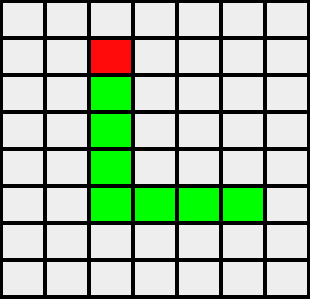
\includegraphics[width=0.20\textwidth, keepaspectratio]{img/pieceLrot0.png} & 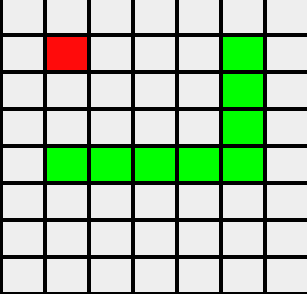
\includegraphics[width=0.20\textwidth, keepaspectratio]{img/pieceLrot3.png}\\
            \end{tabular}
            \begin{tabular}{c}
                Légende:\\
                Rouge: coordonnées où le joueur veut placer la pièce, et indique aussi la case de référence\\
                Vert: pièce L en rotation 0 (img 1) et rotation 3 (img 2)
            \end{tabular}
       \end{table}

       Pour régler ce problème, si la méthode \underline{\textit{ajoutPiece())}} ou \underline{\textit{movePiece()}} est appelé, les coordonnées ("\textit{coo}") reçu en paramètre (clique ou indication de coordonnées en console) sont modifiés. Pour cela, une boucle while est utiliser: tant que les coordonnées Y de la grille de la pièce est de boolean "\textit{false}", les coordonnées ("\textit{coo}") en position Y est diminué de 1, permettant ainsi, si la prochaine case de la grille est de boolean "\textit{true}", de placer la grille de la pièce a partir des coordonnées reçu en paramètre moins 1 .

       \begin{algorithm}[H]\label{alg:whilePlacementPiece}
		         \caption{Boucle while}
                 $posY \leftarrow 0$\;
                 $xx \leftarrow 0$\;
                 $yy \leftarrow 0$\;
                 \While{$!piece.getGrid()[xx][yy+posY]$}{
                    $coo.set(1, coo.get(1)-1)$\;
                    $posY \leftarrow posY+1$\;
				}
			\end{algorithm}

        Cela permet de changer les coordonnées indiquées par le joueur, jusqu'à ce que la valeur des coordonnées de la grille de la pièce est égal a la valeur boolean "\textit{true}".

        \begin{center}
            \begin{tabular}{|m{4.5cm}|m{4.5cm}|m{4.5cm}|}
                \hline
                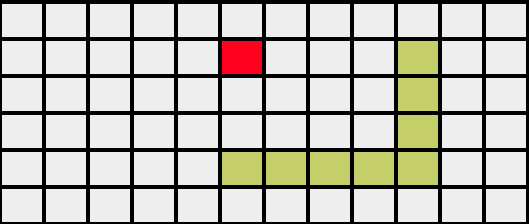
\includegraphics[width=0.20\textwidth, keepaspectratio]{img/pieceLCliqueFantome.png} & 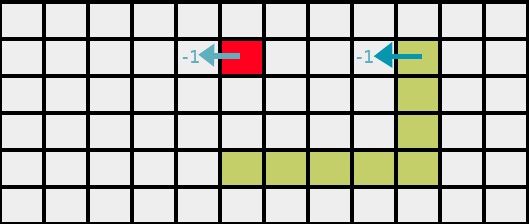
\includegraphics[width=0.20\textwidth, keepaspectratio]{img/pieceLCliqueFantome-1.png} & 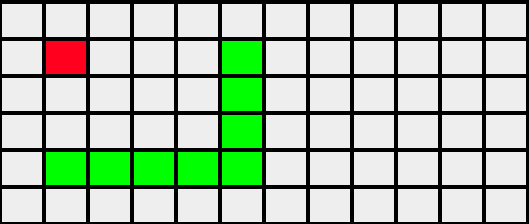
\includegraphics[width=0.20\textwidth, keepaspectratio]{img/pieceLCliqueMis.png}\\
                \hline
                {\small Coordonnées pris en compte} & {\small Boucle while} & {\small Application de l'ajout/déplacement de la pièce}\\
                \hline
            \end{tabular}
        \end{center}

            \begin{tabular}{|m{13.5cm}|}
                \hline
                {\small Légende:}\\
                {\small Rouge: Case de référence et variable "\textit{coo}" qui, sur l'image 1, sont les coordonnées renseignées par le joueur (modifier par la suite dans la while)}\\
                {\small Flèche: Paramètre \textit{coo} (coordonnées) modifié dans la while}\\
                {\small Vert/jaune: Pièce "fantome" où la pièce devrait être normalment sans cette while}\\
                \hline
            \end{tabular}
            \\
            Pendant que la valeur des coordonnées Y de la variable \textit{coo} diminuent, le parcours de la grille de la pièce se fait jusqu'à la case la plus en haut a gauche possible. Donc elle ajoute +1 a la variable \textit{posY}.\\
                \\

                \begin{table}[h]\label{img:prblmPlacementPiece}
                    \begin{tabular}{c}
                        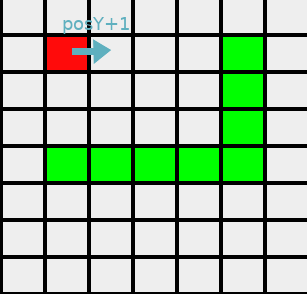
\includegraphics[width=0.20\textwidth, keepaspectratio]{img/pieceLposY.png}
                    \end{tabular}
                    \begin{tabular}{l}
                        {\small Légende:}\\
                        {\small Rouge: Case de référence}\\
                        {\small Flèche: vérification de la prochaine case si sa valeur est "\textit{true}"}\\
                        {\small Vert: pièce L rotation 3}\\
                    \end{tabular}
               \end{table}


      \section{Controleur}

        Le controleur est séparé en plusieurs classes:
        \begin{description}
            \item[classe \textit{PlayMenu}:]{Permet de choisir entre la vue console et la vue graphique.}
            \item[classe \textit{Play}:]{Fait appel aux méthodes du modèle ainsi qu'aux méthodes de choix, en fonction de la vue/joueur actuel.}
            \item[classe \textit{InterfacePlay}:]{Méthodes communes aux choix des joueur: ia ou joueur console.}
            \item[classe \textit{PlayJoueur}:]{Méthodes de choix pour joueur Console, grâce aux Scanner.}
            \item[classe \textit{PlayIa}:]{Méthodes de choix pour ia.}
            \item[enum \textit{EnumAction}:]{Enumère les actions possibles en jeu.}
		\end{description}


        \begin{figure}[H]
			\centering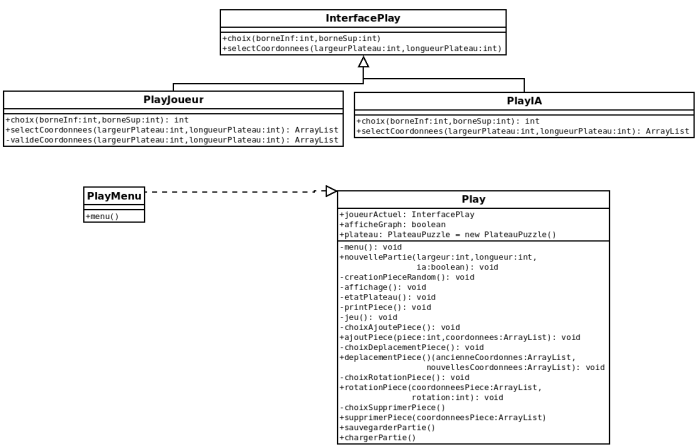
\includegraphics[width=0.64\textwidth, keepaspectratio]{img/diaControleur.png}
			\caption{Controleur}
			\label{fig:diaControleur}
		\end{figure}

        Cette séparations permet simplifier et séparer les choix de jeu. Cela évite la redondance de code.

        \subsection{Controleur : Play}

        En vue console, les choix se font grâce à la variable \textit{joueurActuel} qui est une instance de \textbf{InterfacePlay}. Cela permet, en fonction du choix du joueur (option ia ou non), d'appeller les même méthodes de choix, permettant ensuite d'appeler les méthodes communes à toutes les vues pour accomplir l'action prévu (placer, déplacer...). Tout cela est controlé par la méthode \underline{\textit{jeu()}}.

        \begin{figure}[H]
			\centering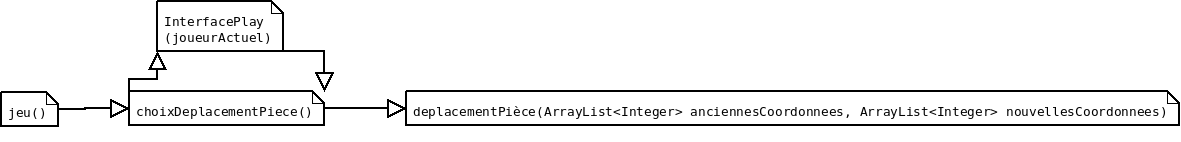
\includegraphics[width=0.64\textwidth, keepaspectratio]{img/graphJoueurChoix.png}
			\caption{Explication choix en fonction du joueur - vue console}
			\label{fig:graphJoueurChoix}
		\end{figure}

        En vue graphique, les choix se font grâce à des actions sur des cases/boutons (cf: voir\ref{subsub:graph}).

        \subsubsection{Controleur : Joueur Ia}\label{subsub:jeuIa}

        Une méthode \underline{\textit{jeuIa()}} est appelé dès que le joueur choisis de regarder l'ia jouer une partie chargé ou une nouvelle partie (en vue graphique ou console). Cette option permet d'avoir une des meilleurs composition de jeu.
        Cette méthode sauvegarde d'abord la partie actuel dans une sauvegarde propre a l'ia. Puis, une boucle "for" lance des \textit{fourmis} (joueur ia qui joue une partie avec des choix random et guidées) afin de faire un certain nombre de parties. A chaque partie, la partie sauvegardée est chargée. L'ia joue et le meilleurs score et le meilleurs plateau généré est enregistré . Cela permet donc d'avoir plusieurs possibilités aléatoires, et d'essayer de trouver la meilleurs composition possible. Cela évite donc de n'avoir qu'une possibilité qui regarde jusqu'à une certaine profondeur.

        La fourmis appel la méthode \underline{\textit{jeu()}}, qui est une commune entre l'ia et le joueur console. Cette méthode permet de choisir l'action que le joueur va effectuer. Il y a un choix a faire, alors cette méthode appel l'attribut \textit{joueurActuel}, permetant de faire un choix random pour l'ia. Pour éviter d'avoir un simple choix aléatoire où toutes les actions ont le même niveau de piorité, une liste d'actions a été créer avec plusieurs même actions à l'interieur. Car, une action pour "avancer" (placer et déplacer) dans le jeu est plus important que de "rester sur place" (rotation dans le plateau et rotation des pièces a jouer) et est plus important qu'une action qui "recule" l'avancement du jeu (supprimer une pièce). La liste peut donc avoir la même actions plusieurs fois, en fonction de son importance dans l'avancement du jeu. Une fois l'action choisis, d'autres méthodes de choix sont appelées en fonction du choix de l'action.

        Pour les actions pour "avancer" dans le jeu, les choix ne sont pas de simple random. En effet, si la fourmis a choisi l'action de PLACER ou DEPLACER une pièce, la méthode \underline{\textit{choixDeplacement()}} ou \underline{\textit{choixAjout()}} est appelée. Ces deux méthodes prenent en compte la largeur, la longueur et le plateau.
        Pour \underline{\textit{choixDeplacement()}}, l'ia choisit d'abord une pièce au hasard sur le plateau, grâce à la méthode \underline{\textit{selectPiece()}} (méthode commune de l'\textbf{InterfacePLay}) qui sélectionne une pièce dans la liste des pièces placer. Les coordonnées récupéré sont les coordonnées de la case de référence de la pièce (cf: voir \ref{img:prblmPlacement}). Une boucle while, presque similaire  à ici\ref{alg:whilePlacementPiece}, est donc nécessaire pour avoir les coordonnées qui aurait pu être cliquées ou indiquées par un véritable joueur. Une fois les coordonnées obtenus, la pièce est supprimé afin d'exercer une simulation de possibilités sans avoir la piècedans le plateau.
        A partir d'ici, \underline{\textit{choixDeplacement()}} exerce comme \underline{\textit{choixAjout()}}. Elle créer une copie du plateau actuel, puis parcours tout le plateau à l'aide des coordonnées placé en clé du HashMap. Si la case est vide et au moins une pièce est situé à 1 ou 2 cases autour de celle ci, alors un test de placement est fait (grâce à la méthode \underline{\textit{validePlacement()}}\ref{txt:validePlacement}). Si ce test est réussi, un deuxième test est necessaire: faire un ajout de la pièce aux coordonnées et calculer le score grâce à la méthode dans la classe \textbf{PlateauPuzzle}). Si le score est supérieur au score du test précédent, une sauvegarde ce celui-ci et des coordonnées est réalisé. Sinon, la boule continue pour les coordonnées suivantes.
        Le \underline{\textit{validePlacement()}} est déjà appellé dans la méthode d'ajout ou de déplacement de la classe \textbf{PlateauPuzzle}, mais cela diminue de temps d'éxecution en vérifiant le placement avant d'appeler la méthode.

        Pour les autres actions (Rotation, Supprimer), le choix est défini en aléatoires.

        Une fois que toutes les fourmis ont finit leurs parties, \underline{\textit{afficheIa()}} affiche le plateau ayant obtenu le meilleurs score. L'affichage déplace d'abord les pièces déjà placer sur le plateau initiale(si c'est une partie charger), puis place ensuite les pièces a jouer en fonction du plateau obtenu par les fourmis. Pour cela, elle utilise les méthodes communes aux différents controleur, pour effectuer des actions.

        \subsubsection{Controleur : Joueur Graphique}\label{subsub:graph}
        Si la vue graphique est choisie, les instances de \textbf{InterfaceGraphique}, \textbf{MouseClicker} et \textbf{ActionGraphique} sont créés a partir du constructeur de la classe \textbf{Play}, permettant ainsi d'afficher la "Vue". Ensuite, la méthode \underline{\textit{menuGraph()}} est appeler, permettant d'appeler \underline{\textit{jeuIa()}} ou \underline{\textit{jeuVue}} en fonction de ce que choisis l'utilisateur. Le choix se fait grâce aux différents boutons. Le joueur peut donc sélectionner la taille de son plateau (via le bouton ligne et colonne qui vont de 5 à 20), charger une partie, afficher le tableau des scores ou encore les règles du jeu. Le fonctionnement des boutons sont assez simple. Le controleur attend que \textbf{ActionGraphique} le notifie, permettant ainsi de récuperer le choix du joueur (via la méthode \underline{\textit{getChoix()}}) et ordonne à la vue ce qu'elle doit faire (afficher la grille, les scores, demander au joueur de selectionné une pièce,...).

        \begin{figure}[H]
            \centering
            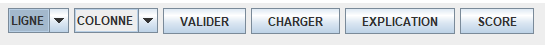
\includegraphics[scale=0.8]{img/menu.png}\label{img:joueurGraphique}
            \caption{Menu principal}
        \end{figure}


    \section{Vue}
        La vue est composé de 3 classes :
        \begin{description}
            \item[classe \textit{InterfaceGraphique}:]{Construit et affiche la vue graphique }
            \item[classe \textit{ActionGraphique}:]{Gère les interactions entre le joueur et la vue}
            \item[classe \textit{MouseClicker}:]{Permet de récupéré les cliques souris du joueur sur la vue}
		\end{description}

		\subsection{InterfaceGraphique}
		L'interface Graphique est composé de nombreuses méthodes pour afficher la vue. La méthode principale est \underline{\textit{buildContentPane()}}.Elle permet à la fenêtre, dans un premier temps, d'afficher le menu principale lorsqu'elle n'a pas de modèle. Ce menu est composé de divers bouton (cf: voir \ref{img:joueurGraphique}). Et quand nous avons un modèle, on affiche la grille en parcourant le plateau et en vérifiant la présence de pièce. Cette grille est une grande fenêtre de couleur noir composé de plusieurs petites fenêtre grise espacé entre-elles, donnant cette impression de grille. On oublie pas d'ajouter à cela les pièces à placer, les boutons de jeu et les rotations des pièces, nous obtenons ceci\ref{img:plateau}.
        Cette classe permet aussi l'affichage des scores, des explications de jeu, des aides, du formulaire pour rentrer son pseudo et des fenêtre de choix.

        \begin{figure}[H]
            \centering
            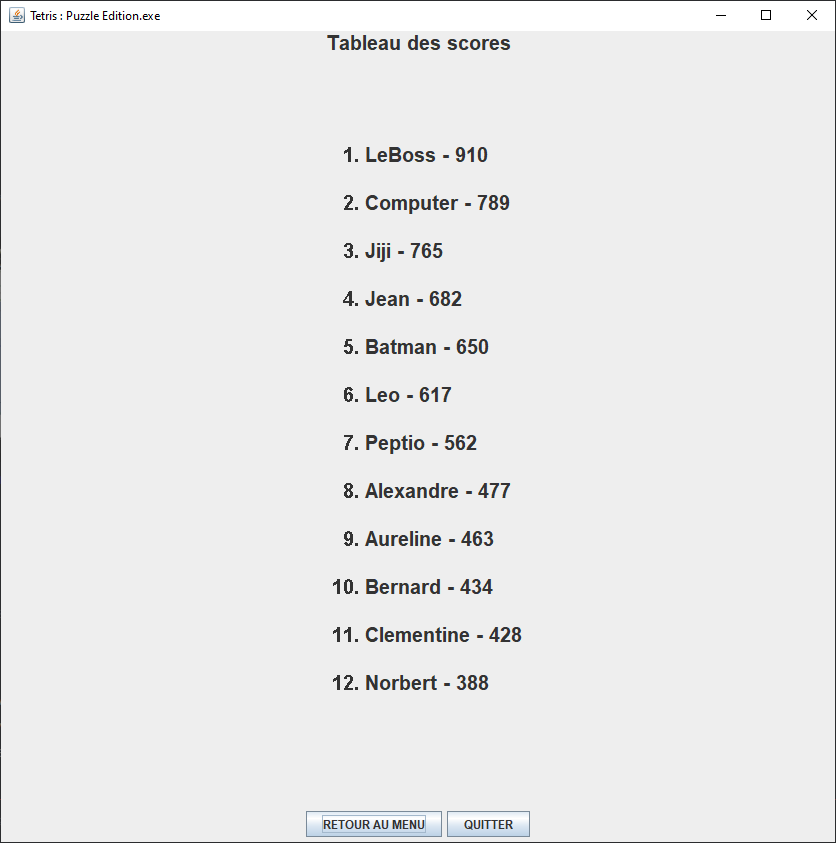
\includegraphics[scale=0.1]{img/score.png}
            \caption{Tableau des scores}
        \end{figure}

        \subsection{ActionGraphique et MouseClicke}
        Ces 2 méthodes sont liés car \textbf{MouseClicker} est utilisé quand les méthodes d'interaction d'\textbf{ActionGraphique} sont appelés. La tache d'\textbf{ActionGraphique} est d'attribuer un rôle à chaque bouton et de gérer l'ordre des évènements quand un joueur veut réaliser une action. Par exemple, le bouton "PLACER" va appeler la méthode \underline{\textit{actionBouton()}} pour vérifier si aucune autre action est en cours. Si oui, on appelle la méthode \underline{\textit{placementPieceVue()}} qui va demander au joueur de sélectionner une pièce. Cette méthode va attendre que \textbf{MouseClicker} lui envoie la pièce sélectionnée pour ensuite demander au joueur de choisir sa rotation et son emplacement. La méthode va de nouveau attendre que \textbf{MouseClicker} lui envoie la case sélectionné. Une fois cette dernière selectionné, les choix sont envoyés au contrôleur dans les méthodes communes d'actions. Pendant les 2 périodes où \textbf{ActionGraphique} attend, une vérification est réalisé afin de contrôler que l'utilisateur n'a pas décidé d'annuler son action. Dans le cas contraire, l'attente est arrété grâce au "break" et la vue est réafficher à son état initiale. Ce processus est semblable pour les méthodes \textit{deplacementPieceVue()} et \textit{supprimerPieceVue()}. Cette class gère aussi les \textbf{Patern} de listener des pièces et des case de la grille, pour que le joueur ne fasse pas de mauvaise sélection.


        \chapter{Conclusion}

	Ce projet était interessant dans l'ensemble. Nous en sommes satisfait, même si l'application peut encore être amélioré, nous avons une vue console et graphique fonctionnelle ainsi qu'un joueur IA un peu plus performant que de simple choix aléatoire.
    Nous avons respecté, dans l'ensemble, ce qui nous avez été demandé, même si nous n'avons pas implementer de patern observeur/observable, nous avons un MVC correct et respecter.

